\section{銀河進化研究の現状 -- 電波領域における多波長・他輝線による銀河の観測的研究 --}\label{galaxy.s1.5}


%%%%%%%%%%%%%%%%%%%%%%%%%%%%%%%%%%%%%%%%%%%%%%%%%%%%%%%%%%%%%%%%%%%%%%%%%%
\subsection{水素原子以外の電波輝線}
%%%%%%%%%%%%%%%%%%%%%%%%%%%%%%%%%%%%%%%%%%%%%%%%%%%%%%%%%%%%%%%%%%%%%%%%%%

水素原子21 cm線以外にも、SKAで観測可能な輝線・吸収線は
多い。中でも特に銀河進化研究の観点から研究の進展が
期待される輝線を表\ref{tab:summary_line}にまとめる。以下では
各項目について簡単な説明を行う。

\begin{table*}[htbp]
\centering
\begin{minipage}{140mm}
\caption{SKAで観測可能なH {\sc i} 21~cm以外の遷移線。}
\label{tab:summary_line}
%\vspace{2mm}
\begin{center}
\begin{tabular}{lccc} \hline
線 & 静止系波長 & 観測可能な赤方偏移$^a$ & 天体の種類\\
 & (GHz) &
\\ \hline
H$_2$O maser & 22 & $>1.2$ & AGN \\
NH$_3$ & 23 & $>1.4$ & ISM \\
%CO & 115 & $>11$ & ISM (in GRB continuum)\\
CO & 115 & $>11$ & ISM (in GRB連続光)\\
\hline
\end{tabular}
\end{center}

$^{a}$遷移線がSKAで観測可能な周波数域
($<10$ GHz)に入る赤方偏移。感度は考慮していない。
\end{minipage}
\end{table*}

\subsubsection{H$_2$Oメーザー}

H$_2$Oメーザーにより、AGN環境(降着円盤やジェット)を調べる
事ができる。
これまでに、$z>0.1$での検出例は2例ある
\citep{2005ApJ...628L..89B,2008Natur.456..927I}
%(type 2 quasar, SDSS J08043+3607 at $z=0.66$と
%lensed type 1 quasar, MG J0414+0534 at $z=2.64$)。
(type 2クエーサー, $z=0.66$にあるSDSS J08043+3607と
lensed type 1クエーサー, $z=2.64$にあるMG J0414+0534)。
後者は重力レンズの効果を受けているが、
レンズの利点は検出が容易になることと、複数の像を
比較する事で小角度の非等方性に制限がつくことである。
レンズによる増光(35倍)を補正すると、後者の天体のフラックス密度は
0.1 mJyのオーダーである。これでも近傍で既に知られている最も
明るいメーザーに比べて2倍明るいので、0.01 mJyのオーダーの感度が出れば
なお良い。SKAレベルの高感度が必要である。

\subsubsection{NH$_3$線}

NH$_3$の様々な($J$, $K$)励起状態を観測する事により、
励起温度を通して星間ガスの温度を見積る事ができる。
同時に、NH$_3$の柱密度も得る事が出来、星間化学反応の
検証をする事もできる。
近傍銀河NGC 253 ($D=3.2$ Mpc)では、NH$_3$輝線の
ピークフラックス密度は0.05 Jy程度である\citep{2005PASJ...57..549T}。
例えば、NGC 253を$z=1$ ($d_\mathrm{L}=6.7$ Gpc)に置くと、
ピークフラックス密度は11 nJyである。これは非常に弱いので、
輝線を観測するよりはむしろ、
強い連続光を背景にして吸収線で観測した方が良いかもしれない。
$z=0.9$の重力レンズクエーサーPKS1830-211では、NH$_3$吸収線
を$(J,\, K)=$ (1, 1)から(10, 10)まで検出し、最大で連続光の2.5\%程度の
吸収が見られた。

\subsubsection{CO吸収線}

分子ガスのトレーサーとしてよく使われるCO($J=1-0$)線は、SKAの
カバーする波長域からは遠いが、高赤方偏移で起るガンマ線バースト
(GRB)等の電波で明るい連続光を背景にした吸収線でなら、
高赤方偏移の分子雲を検出するために用いる事が可能で
ある\citep{2007MNRAS.380.1715I}。
実際、すでに$z=$ 6.3や8.3のGRB電波残光は検出されており、
高赤方偏移の分子ガストレーサーとしてGRB CO吸収線は有望である
\citep{2006ApJ...646L..99F,2010ApJ...712L..31C}。
星間化学反応等を取り入れた
理論計算との比較により、宇宙初期の星間ガスの物理状態や
重元素率のトレーサーとして用いる事が期待される。
連続光のみでなくCO吸収線をも
捉えるのに、SKAの感度が必須である。
10 GHz帯の電波残光は10日後くらいまで徐々に明るくなり
続ける\citep{2007MNRAS.380.1715I}ので、数日の時間スケールで
Time of Opportunity (ToO)観測を許すような
観測態勢が望まれる。 


%%%%%%%%%%%%%%%%%%%%%%%%%%%%%%%%%%%%%%%%%%%%%%%%%%%%%%%%%%%%%%%%%%%%%%%%%%
\subsection{電波連続波で探査する銀河進化史}\label{sec:continuum}
%%%%%%%%%%%%%%%%%%%%%%%%%%%%%%%%%%%%%%%%%%%%%%%%%%%%%%%%%%%%%%%%%%%%%%%%%%

銀河からの電波連続波放射は、主に星形成領域(H \textsc{ii}領域)からの
熱放射(free-free放射)と超新星残骸起源の非熱的放射
(シンクロトロン放射)からなる。ここでは議論を簡単にするために、活動銀河
核起源の電波放射は考えない。
H \textsc{ii}領域も超新星残骸(ここではcore-collapse supernovaeのみを
考える)も比較的寿命の短い大質量星に起因するので、銀河の最近の星形成活動を反映する。
したがって、
銀河の電波連続波光度は、星形成率のよい指標である\citep{1992ARA&A..30..575C}。
すなわち、
%銀河を遠方(高赤方偏移)まで
高赤方偏移の銀河まで
電波連続波で検出できれば、宇宙のどの
時期にどれくらい星が作られてきたか(宇宙の星形成史)を明らかにできる。

電波連続光の光度は、他の良い星形成活動の指標である遠赤外線光度と非常に
良い相関がある事が知られている\citep{1992ARA&A..30..575C,2001ApJ...554..803Y}。少なくとも
近傍銀河については相関は非常に良い。しかし、銀河進化を通して、良い相関が
常に成り立つかどうかは自明ではない。まず、遠赤外線光度は銀河のダストの量
(ダスト・ガス比等)による。したがって、電波・遠赤外線相関もダスト形成史に依って
変化する可能性がある\citep{2013MNRAS.429.3390H}。ダスト形成は、
銀河の化学進化の時間スケールで起こる。一方、電波放射、特に
SKAで観測されるバンドで卓越するシンクロトロン放射は、星間磁場の強度と、
超新星残骸で加速された高エネルギー電子の寿命、および星間空間への拡散の
程度に依存する\citep{2006ApJ...651L.111M}。
星間磁場の強度は、
星間磁場増幅の時間スケールが関わり、高エネルギー電子の寿命は、
高赤方偏移では宇宙背景放射の逆コンプトン散乱によりエネルギーを失う
率が大きくなるので短くなる。つまり、電波・遠赤外線関係は、それの関連する
様々な時間スケールや赤方偏移依存性により、変化する事が期待される。
ところが、現時点では、電波・遠赤外線相関は、中間的な赤方偏移($z\sim 2$)まで
良く成り立っている事が分かってきている
%(例えば、\citep{2002A&A...384L..19G,2003MNRAS.341L...1G,2008MNRAS.386..953I,2009ApJ...706..482M}を参照)。
\citep[e.g.,][]{2002A&A...384L..19G,2003MNRAS.341L...1G,2008MNRAS.386..953I,2009ApJ...706..482M})。
また、$z\sim5$まで成り立っているという報告もある\citep{2010ApJ...712..942M}。

これまでの中間・高赤方偏移での電波・遠赤外線相関の研究は、
感度不足から、非常に明るい銀河に限られ、
銀河進化の一般的描像を得るにはまだほど遠い。遠赤外線では宇宙望遠鏡\textit{Herschel}等で
最近着実に感度を伸ばし、中間赤方偏移までかなり銀河進化の描像は判って
きた\citep{2014MNRAS.441.1017R}。
更に、ALMAによる高赤方偏移銀河からの遠赤外線放射の観測も今後進む事が期待される。
その一方で、電波域の
観測が相対的に立ち後れていると言える。Jansky Very Large Array (JVLA)などに
よる電波連続光の探査観測も計画されているが\citep{2014arXiv1401.4018J}、
SKAなどでさらに「普通の」高赤方偏移銀河を
観測していく事が、一般的な銀河進化の描像を得るためには、必要不可欠である。

銀河のspectral energy distribution (SED)モデルにより、どれくらい遠方まで
電波で星形成銀河が見えるかという予想は、いくつかなされている\citep{2001PASP..113..586T2}。
SKAも含めた将来計画への予想の例を図\ref{fig:murphy}に示す。
この図から、SKAは、既存の装置で最も感度の高いJVLA (図ではEVLA)に比べても
桁で検出限界を押し下げる事が判る。また、ALMAで検出が可能な
$10^{11}L_\odot$程度の遠赤外線光度を持つ銀河を、$z\sim 8$程度まで
検出できる事も見て取れる。更に、可視・近赤外線望遠鏡でサンプルされている
高赤方偏移銀河の電波特性のフォローアップにも、SKAは向いている。

\begin{figure}[tbp]
\begin{center}
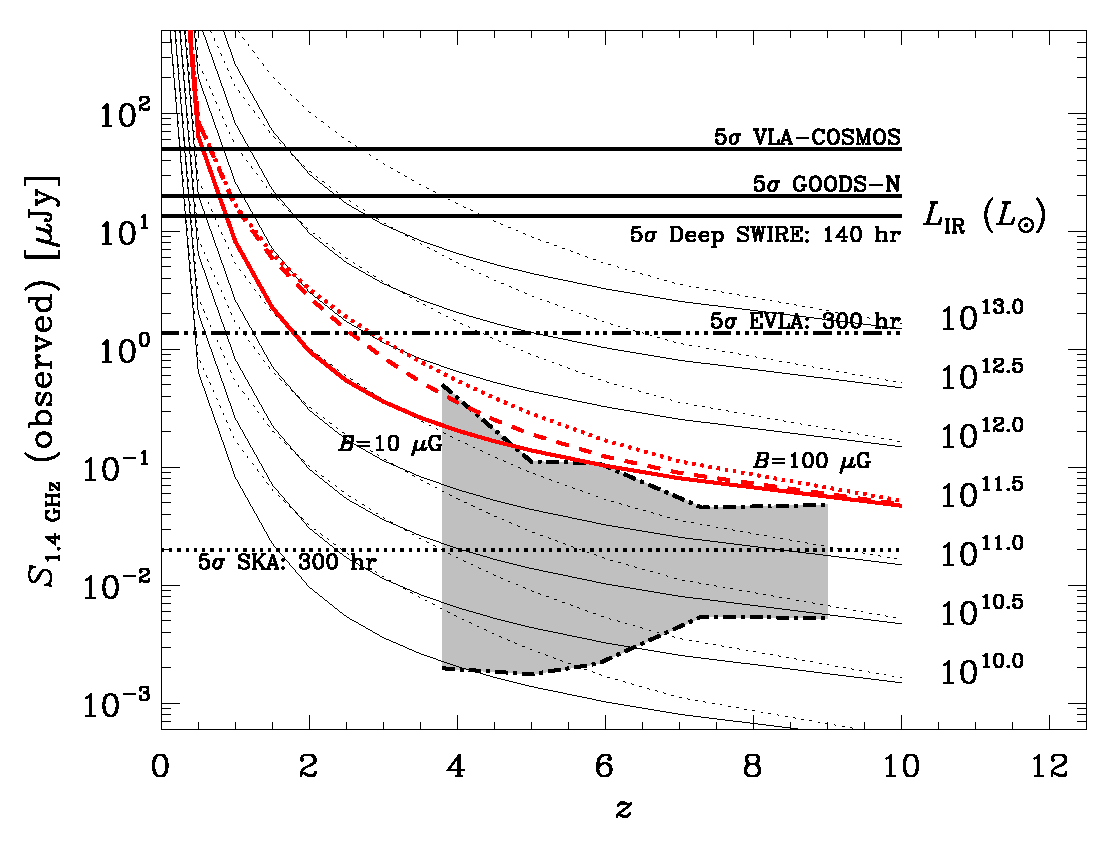
\includegraphics[width=0.8\linewidth]{galaxy/murphy_f3.eps}
\end{center}
\vspace{-0.5cm}
\caption{\citet{2009ApJ...706..482M}より転載。期待される1.4 GHzフラックスを
様々な遠赤外線光度($L_\mathrm{IR}$)の銀河について、赤方偏移の関数として表示したもの。
%
平均的な遠赤外線銀河(LIRG: $L_\mathrm{IR}\sim10^{11.5}$ $L_\odot$、SFR$\sim50$ $M_\odot$ yr$^{-1}$相当)の場合の1.4 GHzフラックスは赤で表している。
%
SEDモデルは、近傍で見られるような電波・遠赤外線相関に基づき、
シンクロトロン放射については、磁場の強度依存性や宇宙背景放射を
逆コンプトン散乱する事による高エネルギー電子のエネルギー減衰
(高赤方偏移で重要)等を
考慮したモデルを用いている。同じ遠赤外線光度について、磁場強度の
異なる場合をプロットしている(実線と点線はそれぞれ10 $\mu$Gと100 $\mu$G;
$L_\mathrm{IR}=10^{11.5}$ $L_\odot$の場合は、破線で磁場強度50 $\mu$Gの場合も
示している)。
又、様々なサーベイ観測の
検出限界も水平線で示されている(式\ref{eq:detection_limit})。灰色に塗られた部分は、
$z\sim 4$--9でのUV光度関数から期待される範囲を示している。
SKAにより初めて、UV (観測される波長では、可視・近赤外線)で
実際に観測されている$z>4$
での銀河種族をサンプル出来る事が判る。また、
$L_\mathrm{IR}=10^{11}$ $L_\odot$といった遠赤外線光度は、ALMAによって観測される
高赤方偏移銀河の典型的限界とも一致する。}
\label{fig:murphy}
\end{figure}

SKAがALMAに対して有利な点は、広い視野である。
ALMAはその視野の狭さから、一般にはサーベイ観測には向かない。
電波で銀河の星形成活動をトレースする意義は、遠赤外線と同様、
ダストによる減光が無視できる点にある。従って、サーベイ観測
という観点からは、SKAはALMAよりも遥かにダスト減光のバイアスの
ない星形成銀河サンプルを得るのに適した望遠鏡であると言える。

積分時間$t_\mathrm{int}$、バンド幅BW、実効的開口面積$A_\mathrm{eff}$、
システム温度$T_\mathrm{sys}$の時、理想的なrmsノイズレベルは
下の様に評価されている\citep{2009ApJ...706..482M}:
\begin{eqnarray}
\left(\frac{\sigma_\mathrm{rms}}{\mathrm{nJy}}\right)\simeq 4
\left(\frac{\mathrm{BW}}{\mathrm{GHz}}\right)^{-1/2}
\left(\frac{t_\mathrm{int}}{300~\mathrm{h}}\right)^{-1/2}
\left(\frac{A_\mathrm{eff}/T_\mathrm{sys}}{15000~\mathrm{m^2~K^{-1}}}\right)^{-1}
\label{eq:detection_limit}
\end{eqnarray}
ここで、$A_\mathrm{eff}/T_\mathrm{sys}=15000~\mathrm{m^2~K^{-1}}$と
BW = 1 GHzは
SKA2で期待される値で、SKA1-MIDでは
$A_\mathrm{eff}/T_\mathrm{sys}=1630~\mathrm{m^2~K^{-1}}$、BW = 770 MHz
である、SKA1-SURVEYでは
$A_\mathrm{eff}/T_\mathrm{sys}=391~\mathrm{m^2~K^{-1}}$、BW = 500 MHzである。
